\section{Introduction}
There are 2 main methods for measuring gloabl bathymetry.
The first is the Smith and Sandwell method which uses sattelite imagery to calculate the elevation of sea mounts \cite{sandwell}.
This method produces accurate results are coarse resolutions.
At finer resolutions this method fails to accurately record measurements.
The best method for measuring fine resolution bathymetry is from ocean surveys.
These surveys are preformed for a wide range of data.
Sediment coposition, biomass, salinity, and bathymetry are a few of the measurements recorded.
These surveys cover a small area and are typically focused to research projects. 
This method produces accurate data, but is very cost and time prohibitive. 
\begin{figure}[hb]
    \centering
    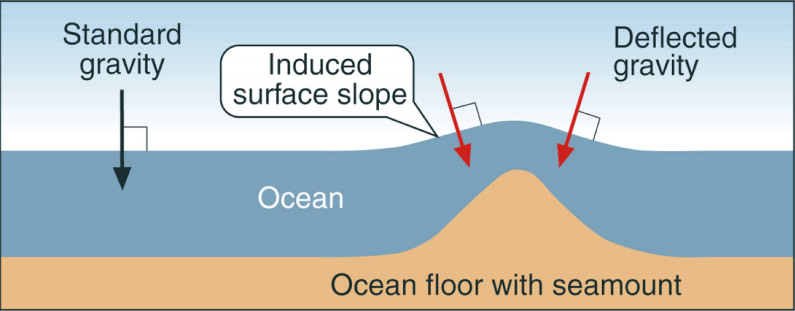
\includegraphics[scale=0.25]{mountainAltimetry}
    \caption{Graphic showing the Smith and Sandwell method}
  \end{figure}

\par
NRL has funded a project titled "Predicting Global Altimetry" lead by geophysicist Dr. Warren Wood.
This project is pioneering the use of machine learning for predicting global ocean bathymetry.
Ideally, these models will produce accurate grids at a fine resolution that is more time and cost prohibitive than ship surveys.
The project is in the early stages of development. 
Currently there is a need to identify appropriate features to predict bathymetry on a global scale. 
The current approach is to preform information gain on many features to then identify ones that will benefit the model.
This creates the need for new features to be discovered and generated. 

\par
The input datasets are in the form of grids that cover area on the earth. 
These grids are point cenetered where the measurement represents a average of the coverage area.
The resolutions for these grids will determine the size and precision of the data.
Grids that cover a wide area are great for representing coarse measurements.
The purpose of predicting accurate bathymetry at a fine level will require features extracted from high resolution grids.
Grid sizes grow quickly as the resolution increases which raises issues with extracting statistics from the set.
